\documentclass[10pt]{article}
\usepackage[margin=1in, paperwidth=8.5in, paperheight=11in]{geometry}
\usepackage{ifpdf,amsmath, amssymb, comment, color, graphicx, stmaryrd,setspace,enumitem,tikz, fancyhdr, wrapfig, textcomp, units, mathptmx, siunitx}

\setlength{\headheight}{14.5pt}
\newcommand{\Q}{\mathbb{Q}}
\newcommand{\R}{\mathbb{R}}
\newcommand{\Z}{\mathbb{Z}}
\newcommand{\vu}{\mathbf{u}}
\newcommand{\vv}{\mathbf{v}}
\newcommand{\vw}{\mathbf{w}}
\newcommand{\vi}{\mathbf{i}}
\newcommand{\vj}{\mathbf{j}}
\newcommand{\vk}{\mathbf{k}}

% Solution text is in red. If you want the solutions to show, remove the \iffalse from the definition of the \red command.
\newcommand{\red}[1]{ %\iffalse
\textcolor{red}{#1} }%\fi}
\newcommand{\blue}[1]{\textcolor{blue}{#1}}
\newcommand{\green}[1]{\textcolor{green}{#1}}
\renewcommand{\section}[1]{\begin{center} \textbf{#1} \\\end{center}}
%
\hyphenpenalty=5000
\setlength{\parindent}{0in}
%\oddsidemargin=-.25in
\allowdisplaybreaks
\pagestyle{fancy}
\renewcommand{\headrulewidth}{0pt}
\lhead{MATH 201}
\rhead{Fall 2019}
%\lfoot{\copyright\ CLEAR Calculus 2010}
\cfoot{}

\begin{document}
%


%\onehalfspacing
\allowdisplaybreaks
%##################################################################
\section{PS\#2: Multivariate functions; vectors - \red{Answer key} }

\begin{enumerate}[leftmargin=0pt]
    \item (ACM 1.1 Exercise 15) The Ideal Gas Law, $PV = RT$, relates the pressure ($P$, in pascals), temperature ($T$, in Kelvin), and volume ($V$, in cubic meters) of 1 mole of a gas ($R = \SI[per-mode=fraction]{8.314}{\J\per\mol\per\K}$ is the universal gas constant), and describes the behavior of gases that do not liquefy easily, such as oxygen and hydrogen. We can solve the ideal gas law for the volume and hence treat the volume as a function of the pressure and temperature:
    \[V(P, T) = \frac{8.314T}{P}.\]
    \begin{enumerate}
        \item Explain in detail what the trace of $V$ with $P = 1000$ tells us about a key relationship between two quantities.
        
        \red{When $P = 1000$, $V(1000, T) = \frac{8.314}{1000} T$. That is, volume increases linearly with temperature, when pressure is held constant. (In fact, even better: volume is \textit{proportional} to temperature if pressure is held constant.)}
        \item Explain in detail what the trace of $V$ with $T = 5$ tells us.
        
        \red{When $T = 5$, $V(P, 5) = \frac{41.57}{P}$. That is, volume is \textit{inversely} proportional to pressure, when temperature is held constant: if the pressure gets higher, the volume gets lower, and if the pressure gets lower, the volume gets higher.}
        \item Explain in detail what the level curve $V = 0.5$ tells us.
        
        \red{If $V = 0.5$:
        \begin{align*}
            0.5 &= \frac{8.314 T}{P}\\
            P &= \frac{8.314}{0.5} T = 16.628 T
        \end{align*}
        This tells us that at constant volume, temperature is proportional to pressure (or, equivalently, pressure is proportional to temperature).
        }
        \item Use 2 or three additional traces in each direction to make a rough sketch of the surface over the domain of $V$ where $P$ and $T$ are each nonnegative. Write at least one sentence that describes the way the surface looks.
        
        \red{Okay, so we've got linear level curves, linear $P$-traces, and $T$-traces that look like $1/P$. So $V$ increases linearly in the $T$ direction, and decreases asymptotically in the $P$ direction. If you look at a graph of $z = x/y$ in CalcPlot3D, restricting the domain to positive numbers, then you'll get a pretty good picture of what's going on here.
        }
        \item Based on all your work above, write a couple of sentences that describe the effects that temperature and pressure have on volume.
        
        \red{Increasing temperature increases volume (proportionally). Increasing pressure decreases volume (in inverse proportion). If we hold volume constant, then increasing temperature increases pressure, and increasing pressure increases temperature.}
    \end{enumerate}
    \item (ACM 1.1 Exercise 16) When people buy a large ticket item like a car or a house, they often take out a loan to make the purchase. The loan is paid back in monthly installments until the entire amount of the loan, plus interest, is paid. The monthly payment that the borrower has to make depends on the amount $P$ of money borrowed (called the principal), the duration $t$ of the loan in years, and the interest rate $r$. For example, if we borrow \$18,000 to buy a car, the monthly payment $M$ that we need to make to pay off the loan is given by the formula \[M(r,t) = \frac{1500r}{1-\frac{1}{\left(1+\frac{r}{12}\right)^{12t}}}.\]
    \begin{enumerate}
        \item Find the monthly payments on this loan if the interest rate is 6\% and the duration of the loan is 5 years.
        
        \red{\[M(0.06, 5) = \frac{1500\cdot 0.06}
        {1-\frac{1}{\left(1+\frac{0.06}{12}\right)^{12\cdot 5}}} = \$347.99.\]
        (Thanks, Wolfram$|$Alpha!)}
        \newpage
        \item Create a table of values that illustrates the trace of $M$ with $r$ fixed at 5\%. Use yearly values of $t$ from 2 to 6. Round payments to the nearest penny. Explain in detail in words what this trace tells us about $M$.
        
        \red{
        \[
        \begin{array}{c|c|c|c|c|c}
            t          & 2        & 3        & 4        & 5        & 6        \\
            \hline
            M(0.05, t) & \$789.69 & \$539.48 & \$414.53 & \$339.68 & \$289.89
        \end{array}
        \]
        So this tells us that at a fixed interest rate, extending the loan duration decreases the monthly payments (in fact, by a decreasing amount).
        }
        \item Create a table of values that illustrates the trace of $M$ with $t$ fixed at 3 years. Use rates from 3\% to 11\% in increments of 2\%. Round payments to the nearest penny. Explain in detail what this trace tells us about $M$.
        
        \red{
        \[
        \begin{array}{c|c|c|c|c|c}
            r       & 3\%      & 5\%      & 7\%      & 9\%      & 11\%     \\ \hline
            M(r, 3) & \$523.46 & \$539.48 & \$555.79 & \$572.40 & \$589.30
        \end{array}
        \]
        So this tells us that at a fixed loan duration, increasing the interest rate increases the monthly payment (in fact, by an amount that is sliiiiiiightly increasing).
        }
        \item Consider the combinations of interest rates and durations of loans that result in a monthly payment of \$200. Solve the equation $M(r, t) = 200$ for $t$ to write the duration of the loan in terms of the interest rate. Graph this level curve and explain as best you can the relationship between $t$ and $r$.
        
        \red{ We did some algebra in class for this:
        \begin{align*}
            200 &= \frac{1500r}{1-\frac{1}{\left(1+\frac{r}{12}\right)^{12t}}}\\
            200\left[1-\left(1+\frac{r}{12}\right)^{-12t}\right] &= 1500r \\
            1-\left(1+\frac{r}{12}\right)^{-12t} &= 7.5 r \\
            1-7.5r &= \left(1+\frac{r}{12}\right)^{-12t}\\
            \ln(1-7.5r) &= -12t \cdot \ln\left(1+\frac{r}{12}\right) \\
            t &= \frac{\ln(1-7.5r)}{-12\ln\left(1+\frac{r}{12}\right)}
        \end{align*}
        Okay, so that's a perfectly fine function of $r$ that we now have for $t$. We can graph it:\\
        \begin{center}
            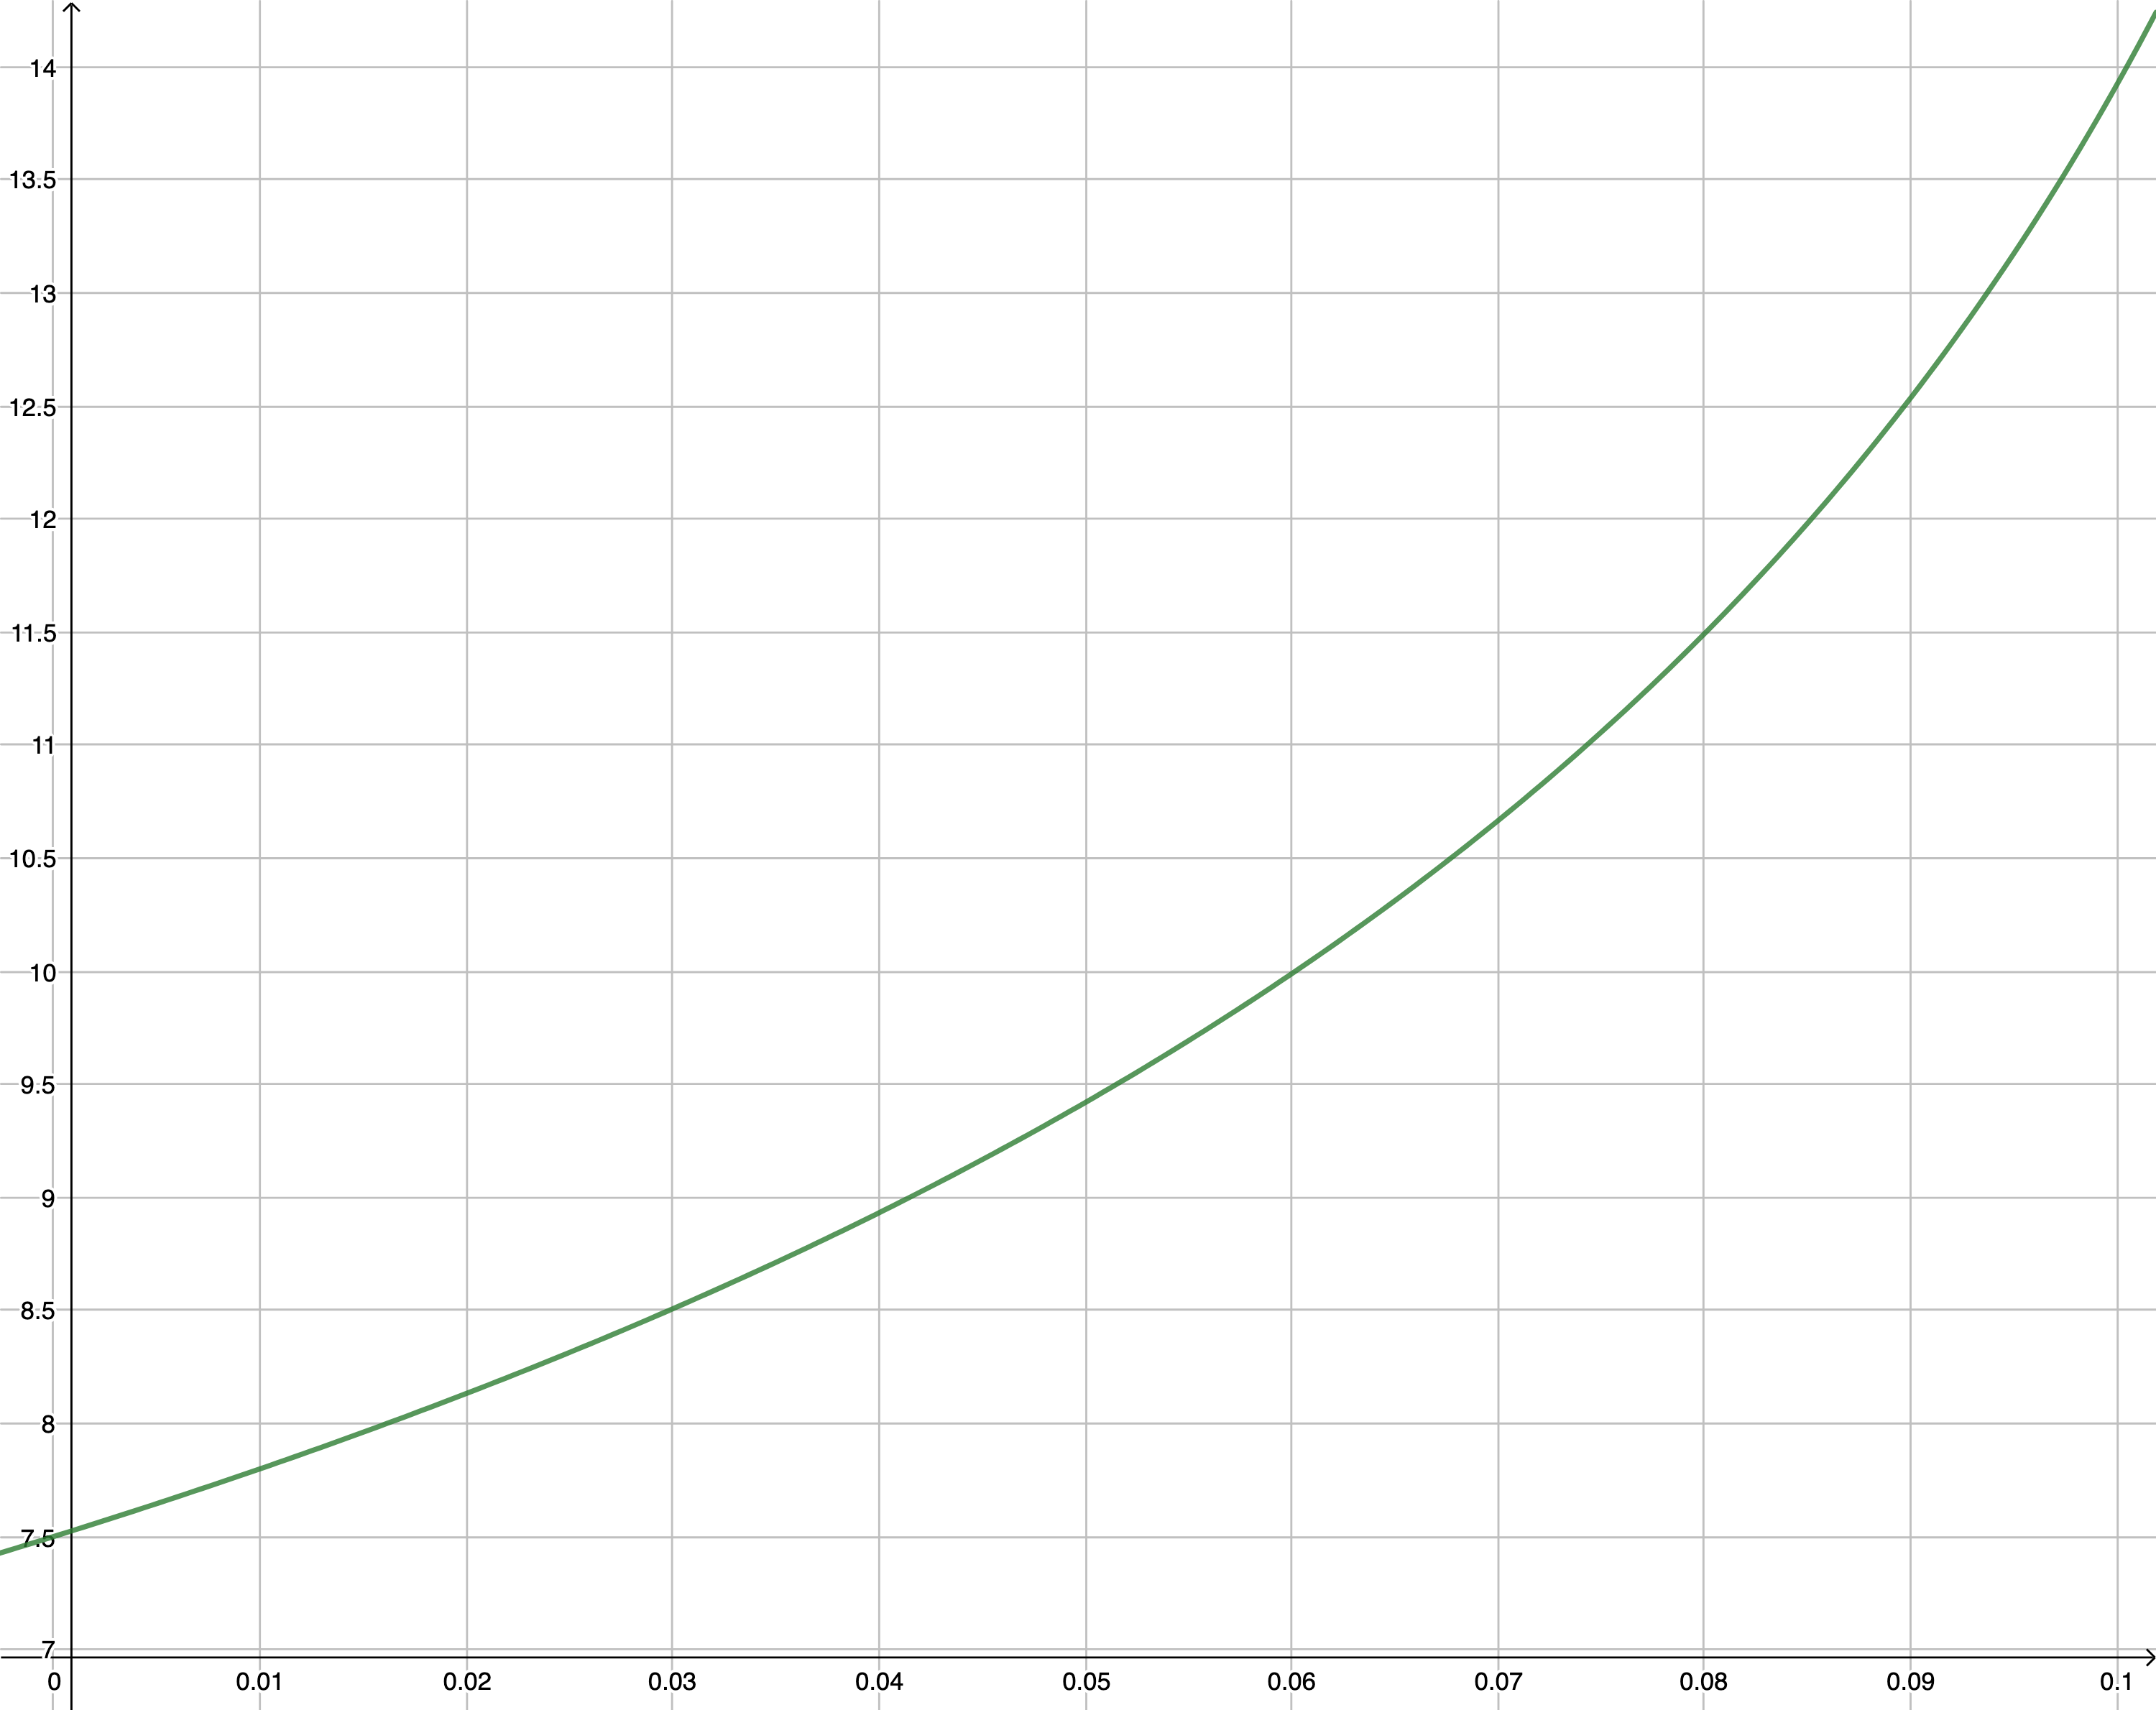
\includegraphics[scale=0.09]{geogebra-export.png}\\
        \end{center}
        (I used Geogebra to generate this graph, because Wolfram$|$Alpha insisted that the graph should be polar since it involved an $r$, and I couldn't figure out a good way to tell it that no, honestly, this is a rectangular plot, just with weird variable letters.)\\
        So, if we want to have a fixed monthly payment of \$200, then increasing the duration will force us to increase the interest rate, and increasing the interest rate will force us to increase the duration.\\
        (In other words that are more practical: if we're offered a lower interest rate and we want to keep our payments the same, then we can pay off the loan in a shorter duration.)}
    \end{enumerate}
    \item 
    \begin{minipage}[t]{0.5\linewidth}
    (ACM 1.2 Exercise 16)
    A force (like gravity) has both a magnitude and a direction. If two forces $\vu$ and $\vv$ are applied to an object at the same point, the resultant force on the object is the vector sum of the two forces. When a force is applied by a rope or a cable, we call that force \textit{tension}. Vectors can be used to determine tension.
    
    As an example, suppose a painting weighing 50 pounds is hung from a wire attached to a hook which is not perfectly centered on the picture, as illustrated in the figure. We need to know how much tension will be on the wire to know what kind of wire to use to hang the picture. Assume the hook is on the picture frame at point $O$. Let $\vu$ be the vector emanating from point $O$ to the left and $\vv$ the vector emanating from point $O$ to the right. Assume $\vu$ makes a $30^\circ$ angle with the horizontal at point $O$ and $\vv$ makes a $45^\circ$ angle with the horizontal at point $O$. Our goal is to determine the vectors $\vu$ and $\vv$.
    \end{minipage}
    \hspace{0.1in}
    \begin{minipage}[t]{0.4\linewidth}
    \vspace{0pt}
    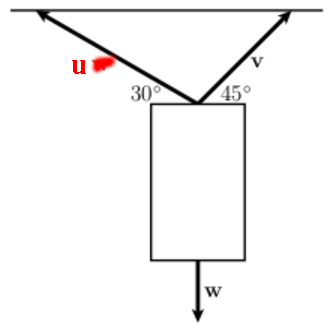
\includegraphics[width=\linewidth]{fig_9_2_forces.pdf}
    \end{minipage}
    \begin{enumerate}
        \item Treat point $O$ as the origin. Use trigonometry to find the components $u_1$ and $u_2$ so that $\vu = u_1 \vi + u_2 \vj$. Since we don't know the magnitude of $u$, your components will be in terms of $|\vu|$ and the cosine and sine of some angle. The find the components $v_1$ and $v_2$ so that $\vv =v_1 \vi + v_2 \vj$. Again, your components will be in terms of $|\vv|$ and the cosine and sine of some angle.
        
        \red{Note that in this situation, positive $\vi$ points to the right and positive $\vj$ points up.\\
        By trigonometry, the horizontal component of $\vu$ is $|\vu|\cos30^\circ$, and the vertical component is $|\vu|\sin30^\circ$. So, $\vu = -|\vu|\cos30^\circ \vi + |\vu|\sin30^\circ \vj$. (Note the negative sign on the first component, so that $\vu$ points left.)\\
        Similarly, $\vv = |\vv|\cos45^\circ \vi + |\vv|\sin45^\circ \vj$. (No negatives this time.)
        }
        \item The total force holding the picture up is given by $\vu + \vv$. The force acting to pull the picture down is given by the weight of the picture. Find the force vector $\vw$ acting to pull the picture down.
        
        \red{Since the picture weighs 50 pounds, $\vw = -50\vj$.}
        \item The picture will hang in equilibrium when the force acting to hold it up is equal to the force acting to pull it down. Equate these forces to find the components of the vectors $\vu$ and $\vw$.
        
        \red{The text of this question is slightly misleading: it suggests that we want $\vu + \vv = \vw$. If you work this all out, you'll get negative values for the magnitudes of $\vu$ and $\vv$, which clearly doesn't make sense. Instead what we want is $\vu + \vv = -\vw$, because the resultant tension force should act to counter the weight of the picture.
        So, we want $(-|\vu|\cos30^\circ \vi + |\vu|\sin30^\circ \vj) + (|\vv|\cos45^\circ \vi + |\vv|\sin45^\circ \vj) = 0 \vi + 50 \vj$. Equating the $\vi$ and $\vj$ components:
        \begin{align*}
            -|\vu|\cos30^\circ + |\vv|\cos45^\circ &= 0 \\
             |\vu|\sin30^\circ + |\vv|\sin45^\circ &= 50
        \end{align*}
        Now we have a system of two equations in two unknowns, $|\vu|$ and $|\vv|$. The solution of this system will require some tedious algebra, which I'm happy to feed to Wolfram$|$Alpha (using $u$ to mean $|\vu|$ and similar for $v$):
        \\
        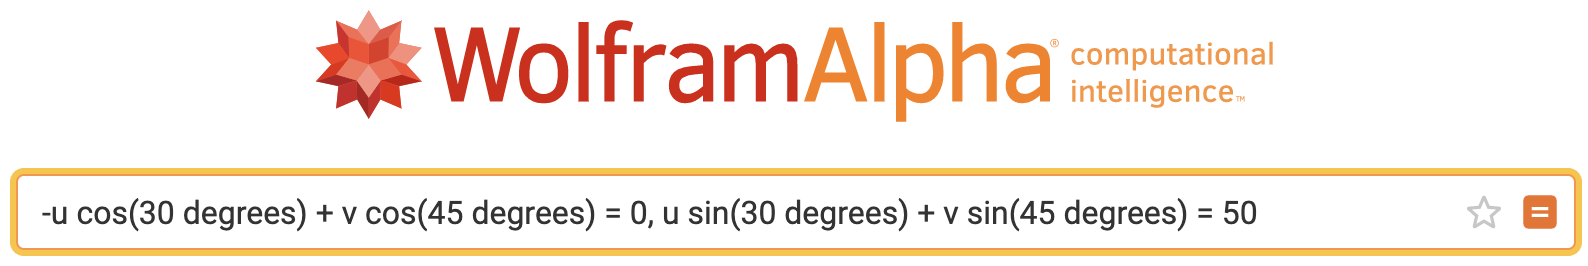
\includegraphics[width=\linewidth]{wa-3-1.png} \\
        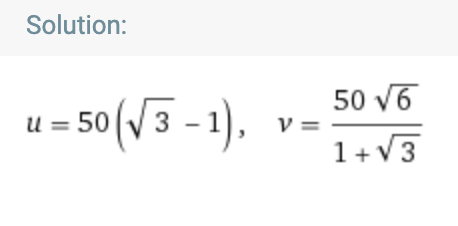
\includegraphics[width=0.4\linewidth]{wa-3-2.png}
        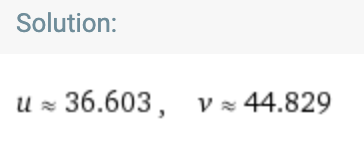
\includegraphics[width=0.4\linewidth]{wa-3-3.png}\\
        Thanks, Wolfram$|$Alpha! Therefore:
        \begin{align*}
            \vu &= - 50(\sqrt{3} - 1) \cos30^\circ \vi + 50(\sqrt{3} - 1) \sin30^\circ \vj\\
            &\approx -31.699 \vi + 18.301 \vj \\
            \vv &= \frac{50\sqrt{6}}{1+\sqrt{3}}\cos45^\circ\vi + \frac{50\sqrt{6}}{1+\sqrt{3}}\sin45^\circ\vj\\
            &\approx 31.699 \vi + 31.699 \vj.
        \end{align*}
        }
    \end{enumerate}
\end{enumerate}

\red{\textbf{Learning Targets}: Your work on this assignment might reasonably be construed to hit Learning Targets HBT1,2,3 (if you used a computer to help with your work), V1 and maybe V2, S1 and S2.}

\end{document}